%
% fig-integral.tex -- Integral der geometrischen Reihe
%
% (c) 2026 Prof Dr Andreas Müller
%
\begin{figure}
\centering
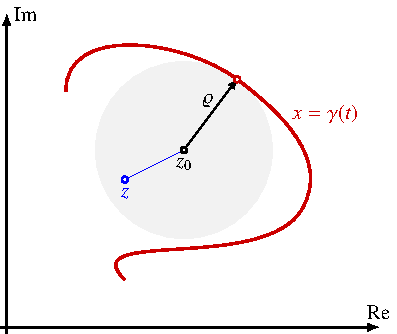
\includegraphics{chapters/040-analytisch/images/integral.pdf}
\caption{Durch Integration der geometrischen Reihe um den Punkte $z_0$
entlang eines nicht notwendigerweise geschlossenen Pfades $\gamma$ 
entsteht aus einer stetigen Funktion $g(x)$ auf der Kurve eine im
Komplement der Kurve holomorphe Funktion $f(z)$.
Um den Punkt $z_0$ kann für $f(z)$ eine eine Potenzreiheentwicklung 
angegeben werden kann, die als Konvergenzradius den minimalen
Abstand $\varrho$ zur Kurve hat.
\label{buch:analytisch:fig:integral}}
\end{figure}
